% !TeX spellcheck = ru_RU
% !TEX root = vkr.tex

\section{Проектирование решения}

После полученных результатов команда \verb|TATLIN.BACKUP| провела эксперименты, где так же стало очевидно преимущество использования нескольких рантаймов с точки зрения пропускной способности.

Однако, неясным осталась надежность такой системы: разработчики tokio не дают никаких гарантий относительно взаимодействия такой системы, а наоборот утверждают, что при некотором обращении с такой конструкцией могут быть наблюдаемы падения производительности или достижимо неопределенное поведение. \verb|TATLIN.BACKUP| позиционирует себя как высоконадежное производительное решение, а потому использовать в нем конструкцию без гарантий не возможно.

\subsection{Шардирование глобальной очереди}

Если дублировать весь рантайм нельзя, вероятно, уменьшить ограничение накладываемое глобальной очередью получится при использовании нескольких глобальных очередей в одном рантайме, как представленно на изображении~\ref{fig:tokio:duplicated_arch}.

\begin{figure}[H]
    \begin{center}
        \makebox[\textwidth]{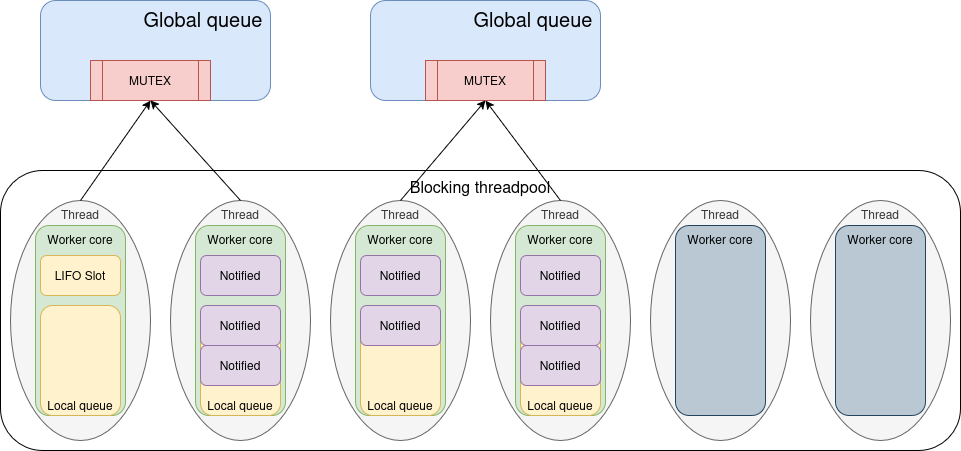
\includegraphics[scale=0.55]{pictures/tokio_duplicated.drawio.png}}
    \end{center}

    \caption{Упрощенное представление многопоточного рантайма}
    \label{fig:tokio:duplicated_arch}
\end{figure}
Здесь и далее под рабочей группой будет пониматься глобальная очередь с фиксированным количеством воркеров.

Это было реализовано с следующими измененями в интерефейсе tokio:

\begin{itemize}

\item При создании рантайма пользователь специфицирует количество групп (\verb|worker_groups|) и количество воркеров в каждой группе (\verb|worker_threads|). В результате рантайм инстанциируется с \verb|worker_threads| * \verb|worker_groups| системными потоками для исполнения асинхронных замыканий.
\item Для отправки замыкания исполняться в определенную рабочую группу добавлен метод \verb|tokio::spawn_into|.
\end{itemize}


Рабочая группа выбирается с помощью локального для потока рандома~\cite{xorshiftRNG} в следующих случаях:

\begin{itemize}
    \item Создании задачи с в процессе аллокации замыкания с методом \verb|tokio::spawn|
    \item Отправки \verb|Notified| в планировщик tokio в следствии готовности системных ресурсов
\end{itemize}

Каждая группа изолирована от остальных, то есть воркеры не могут похищать задачи из глобальных очередей или локальных очередей воркеров из других групп. Это вынуждает их быть запаркованными при нехватке задач в собственной группе, что позволяет:

\begin{itemize}
    \item Избежать конфликтов между воркерами из различных групп.
    \item Экономить системные ресурсы.
\end{itemize}

При появлении задач будет разбужено соответствующее количество воркеров в соответствующей группе.

\subsection{Индентификатор задач}

При создании задачи для нее генерируется индентификатор на одной статической ячейке памяти, переменной разделяемой между всеми попытками создать задачу в рамках процесса. То есть при создании каждой задачи, пусть даже в различных потоках, устанавливается глобальный порядок на одной ячейке памяти для поддержания уникальности индентификаторов.

Этого можно избежать если, индентификатор будет состоять из двух частей как представлено на листинге~\ref{listing:id:composite} --- в таком случае можно инстанциировать несколько производителей различных индентификаторов.

\begin{listing}[H]
    \begin{minted}{rust}
struct Id {
    head: u64,
    tail: u64,
}
    \end{minted}

    \caption{Асинхронное замыкание}
    \label{listing:id:composite}
\end{listing}

А именно: на статической атомарной перменной будет производиться генерации первой части индентификатора задачи, так называемого индентификатора производителя индентификаторов задач, представленного на листинге~\ref{listing:id:provider}

\begin{listing}[H]
    \begin{minted}{rust}
struct IdProvider {
    head: u64,
    tail_counter: AtomicU64,
}
    \end{minted}

    \caption{Асинхронное замыкание}
    \label{listing:id:provider}
\end{listing}

каждый из которых будет иметь собственную атомарную ячейку памяти для генерации индентификаторов задач.

При создании задачи ее необходимо зарегистрировать в \verb|OwnedTasks|, путем выбора шарда и помещению в него указателя \verb|Task|. Выбор шарда ранее происходил с помощью индентификатора задачи, то есть использование шардов происходило последовательно. Однако, при использовании составного индентификатора повышается возможность конфликта при выборе шарда, что значительно снижает производительность. Поэтому в данный момент применение составному индентификатору не найдено.
